\setcounter{chapter}{2}
\chapter{Circuiti Elettrici}

\section{Condensatori}

In generale un condensatore \`e una coppia di conduttori che hanno carica Q e -Q rispettivamente. Un  esempio \`e dato da due piani conduttori in parallelo.

\subsection{Condensatore a piani paralleli}

\begin{wrapfigure}{r}{0.4\textwidth} % 'r' for right, 'l' for left
    \centering
    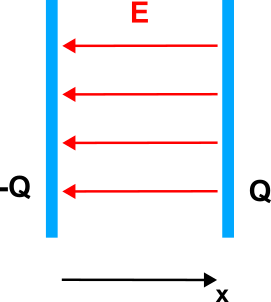
\includegraphics[width=0.3\textwidth]{images/parallelcapac} % Replace with your image
\end{wrapfigure}
Consideriamo due piani conduttori posti in parallelo come in figura, e assumiamo che la distanza $d$ tra i piani sia molto pi\`u piccola di $\sqrt{A}$ dove $A$ \`e l'area delle superfici planari. Imporre una condizione del genere ci permette di considerare gli effetti che si generano al bordo dei piatti e quindi possiamo assumere che il campo elettrico che generato nella regione tra i due piani coincide con quello che si avrebbe se le superfici avessero una estensione infinita. Il campo elettrico \`e dato da 
\begin{equation*}
	\bold{E} = -\frac{\sigma}{\varepsilon_0} \bold{\hat{x}}
\end{equation*}
dove $\sigma = Q/A$ e il campo ha direzione opposta a quella dell'asse $x$. Definiamo \textit{capacitanza} la grandezza 
\begin{equation}
	C = \frac{Q}{V}
\end{equation}
dove V rappresenta il $voltaggio$ o la \textit{differenza di potenziale}, tra i due piani paralleli. Dato che $\bold{E} = -\frac{d\phi}{dx}$, avremo che 
\begin{equation*}
	\phi(x) =-Ex+c \quad \Rightarrow \quad V = \phi(0) - \phi(d) = Ed = \frac{Qd}{A \varepsilon_0}
\end{equation*} 
e  quindi possiamo concludere che la capacitanza per due piatti paralleli di area A e posti ad una distanza $d$, sono
\begin{equation*}
	C = \frac{A \varepsilon_0}{d}
\end{equation*}
La capacitanza di un condensatore dipende dalla sua geometria e non dalla carica Q. I condensatori in generale vengo usati per immagazzinare energia elettrica. L'energia accumulabile da un condensatore \`e data dalla relazione 
\begin{equation*}
	U = \frac{1}{2} \varepsilon_0 \int_V dV \; \bold{E} \cdot \bold{E} = \frac{A \varepsilon_0}{2} \int_{0}^{d} dx \; \left ( \frac{\sigma}{\varepsilon_0}\right)^2 = \frac{Q^2}{2C}
\end{equation*}
L'unit\`a di misura per la capacitanza \`e data dal \textit{Farad} che \`e dato da 
\begin{equation*}
	[F] = \frac{[Coulomb]}{[Volt]}
\end{equation*}

\subsection{Conduttori con condensatore interno}
\subsection{Sistemi di conduttori / condensatore a pi\u strati}
\section{Conduttori Ohmnici}
\subsection{Legge di Ohm}

\section{Componenti di un circuito elettrico}
\subsection{Resistenze in serie e parallelo}
\subsection{Condensatori in serie e parallelo}
\subsection{Riduzione di un circuito}
\subsection{Legge di Kirchoff}

\section{Carica e Scarica di un condensatore}
\section{Forza elettromotrice}


